
%(BEGIN_QUESTION)
% Copyright 2006, Tony R. Kuphaldt, released under the Creative Commons Attribution License (v 1.0)
% This means you may do almost anything with this work of mine, so long as you give me proper credit

Det er et problem en eller annen plass i dette væskestrømningsreguleringssystemet. Regulatoren er i auto-modus, med et settpunkt på  65\%, men likevell viser FT og FIC 0.3\% (nesten ingen strømning). 
%There is a problem somewhere in this liquid flow control system.  The controller is in automatic mode, with a setpoint of 65\%, yet the flow indicator and the flow controller both register 0.3\%: (nearly) zero flow.  A P\&ID of the loop appears here:

$$\includegraphics[width=15.5cm]{i02518x01.eps}$$

Forklar hvordan du ville feilsøkt i dette systemet, og hvilke mulige feil som kan forårsake at regulatorn ikke klarer å holde settpunktet. 

%Explain how you would begin troubleshooting this system, and what possible faults could account for the controller not being able to maintain liquid flow at setpoint.

\vskip 20pt \vbox{\hrule \hbox{\strut \vrule{} {\bf Suggestions for Socratic discussion} \vrule} \hrule}

\begin{itemize}
\item{} Explain how you could divide this control system into distinct areas or zones which you may then begin to refer to when ``dividing and conquering'' the problem. 
\end{itemize}

\underbar{file i02518}
%(END_QUESTION)





%(BEGIN_ANSWER)

One possible fault has to do with the control valve: perhaps something has happened to make it fail closed (loss of air supply, signal, etc.).  Other possible problems include the following:

\begin{itemize}
\item{} Pump not running (no source of fluid power to motivate flow)\
\item{} Very poor controller tuning
\item{} Wrong controller action
\item{} Valve failed closed (loss of air supply, signal, etc.)
\item{} Transmitter failed, showing no flow when in fact there is
\end{itemize}

A good ``first test'' for troubleshooting the loop is to check the controller output: is it trying to open up the valve?


%(END_ANSWER)





%(BEGIN_NOTES)

\vskip 20pt \vbox{\hrule \hbox{\strut \vrule{} {\bf Virtual Troubleshooting} \vrule} \hrule}

This question is a good candidate for a ``Virtual Troubleshooting'' exercise.  Presenting the diagram to students, you first imagine in your own mind a particular fault in the system.  Then, you present one or more symptoms of that fault (something noticeable by an operator or other user of the system).  Students then propose various diagnostic tests to perform on this system to identify the nature and location of the fault, as though they were technicians trying to troubleshoot the problem.  Your job is to tell them what the result(s) would be for each of the proposed diagnostic tests, documenting those results where all the students can see.

During and after the exercise, it is good to ask students follow-up questions such as:

\begin{itemize}
\item{} What does the result of the last diagnostic test tell you about the fault?
\item{} Suppose the results of the last diagnostic test were different.  What then would that result tell you about the fault?
\item{} Is the last diagnostic test the best one we could do?
\item{} What would be the ideal order of tests, to diagnose the problem in as few steps as possible?
\end{itemize}

%INDEX% Basics, control loop troubleshooting: determining cause of control problem

%(END_NOTES)


